\documentclass[border=10pt, tikz]{standalone}
\usepackage[T1]{fontenc}
\usepackage{helvet}
\renewcommand{\familydefault}{\sfdefault}
\usepackage{amsmath, amssymb}
\usetikzlibrary{arrows.meta, positioning, calc, backgrounds, fit}

\definecolor{slateDark}{HTML}{0F172A}
\definecolor{slateText}{HTML}{334155}
\definecolor{slateMuted}{HTML}{64748B}
\definecolor{slateBorder}{HTML}{CBD5E1}
\definecolor{slateBg}{HTML}{F8FAFC}

\definecolor{redDark}{HTML}{991B1B}
\definecolor{redMain}{HTML}{DC2626}
\definecolor{redBg}{HTML}{FEF2F2}

\definecolor{blueDark}{HTML}{0369A1}
\definecolor{blueMain}{HTML}{0284C7}
\definecolor{blueBg}{HTML}{F0F9FF}

\definecolor{greenDark}{HTML}{047857}
\definecolor{greenMain}{HTML}{059669}
\definecolor{greenBg}{HTML}{ECFDF5}

\begin{document}
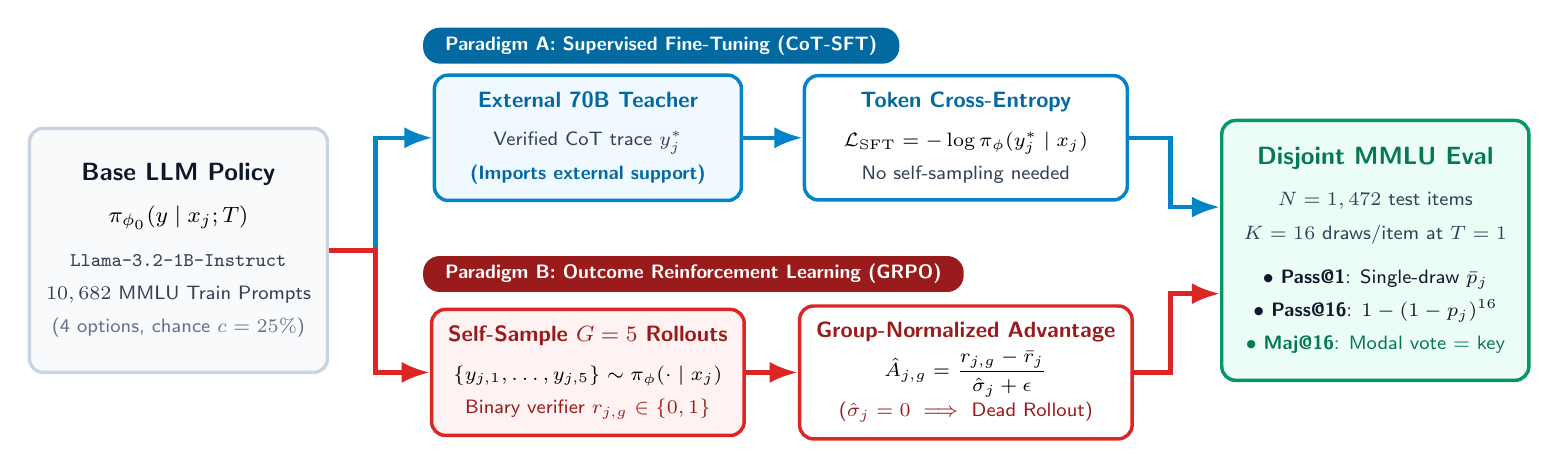
\begin{tikzpicture}[
    >=Latex,
    font=\sffamily,
    box/.style={
        rectangle,
        rounded corners=5pt,
        draw=#1,
        line width=1.25pt,
        fill=white,
        align=center,
        inner sep=6pt
    },
    pill/.style={
        rectangle,
        rounded corners=6pt,
        fill=#1,
        text=white,
        font=\sffamily\bfseries\scriptsize,
        inner xsep=8pt,
        inner ysep=3pt
    },
    arrow/.style={
        ->,
        line width=1.6pt,
        color=#1
    }
]

% Left: Base Model + Prompt
\node[box=slateBorder, fill=slateBg, minimum width=3.5cm, minimum height=3.1cm] (base) at (-7.4, -0.05) {
    \textbf{\small\color{slateDark} Base LLM Policy}\\[3pt]
    {\footnotesize $\pi_{\phi_0}(y \mid x_j; T)$}\\[4pt]
    {\scriptsize\color{slateText} \texttt{Llama-3.2-1B-Instruct}}\\
    {\scriptsize\color{slateText} $10,682$ MMLU Train Prompts}\\
    {\scriptsize\color{slateMuted} (4 options, chance $c=25\%$)}
};

% Top Branch: CoT-SFT
\node[pill=blueDark, anchor=west] at (-4.3, 2.55) {Paradigm A: Supervised Fine-Tuning (CoT-SFT)};

\node[box=blueMain, fill=blueBg, minimum width=3.9cm, minimum height=1.35cm] (sft1) at (-2.2, 1.38) {
    \textbf{\footnotesize\color{blueDark} External 70B Teacher}\\[2pt]
    {\scriptsize\color{slateText} Verified CoT trace $y^*_j$}\\
    {\scriptsize\color{blueDark} \textbf{(Imports external support)}}
};

\node[box=blueMain, fill=white, minimum width=4.1cm, minimum height=1.35cm] (sft2) at (2.6, 1.38) {
    \textbf{\footnotesize\color{blueDark} Token Cross-Entropy}\\[2pt]
    {\scriptsize $\mathcal{L}_{\mathrm{SFT}} = -\log \pi_\phi(y^*_j \mid x_j)$}\\
    {\scriptsize\color{slateText} No self-sampling needed}
};

% Bottom Branch: GRPO
\node[pill=redDark, anchor=west] at (-4.3, -0.35) {Paradigm B: Outcome Reinforcement Learning (GRPO)};

\node[box=redMain, fill=redBg, minimum width=3.9cm, minimum height=1.45cm] (rl1) at (-2.2, -1.6) {
    \textbf{\footnotesize\color{redDark} Self-Sample $G=5$ Rollouts}\\[2pt]
    {\scriptsize $\{y_{j,1},\dots,y_{j,5}\} \sim \pi_\phi(\cdot\mid x_j)$}\\
    {\scriptsize\color{redDark} Binary verifier $r_{j,g} \in \{0,1\}$}
};

\node[box=redMain, fill=white, minimum width=4.1cm, minimum height=1.45cm] (rl2) at (2.6, -1.6) {
    \textbf{\footnotesize\color{redDark} Group-Normalized Advantage}\\[2pt]
    {\scriptsize $\hat{A}_{j,g} = \dfrac{r_{j,g} - \bar{r}_j}{\hat{\sigma}_j + \epsilon}$}\\[1pt]
    {\scriptsize\color{redDark} ($\hat{\sigma}_j = 0 \implies$ Dead Rollout)}
};

% Right: Disjoint Evaluation Bank
\node[box=greenMain, fill=greenBg, minimum width=3.9cm, minimum height=3.3cm] (eval) at (7.8, -0.05) {
    \textbf{\small\color{greenDark} Disjoint MMLU Eval}\\[3pt]
    {\scriptsize\color{slateText} $N = 1,472$ test items}\\
    {\scriptsize\color{slateText} $K = 16$ draws/item at $T=1$}\\[4pt]
    {\scriptsize\color{slateDark} $\bullet$ \textbf{Pass@1}: Single-draw $\bar{p}_j$}\\
    {\scriptsize\color{slateDark} $\bullet$ \textbf{Pass@16}: $1-(1-p_j)^{16}$}\\
    {\scriptsize\color{greenDark} $\bullet$ \textbf{Maj@16}: Modal vote $=$ key}
};

% Arrows
\draw[arrow=blueMain] (base.east) -- (-4.9, -0.05) |- (sft1.west);
\draw[arrow=blueMain] (sft1.east) -- (sft2.west);
\draw[arrow=blueMain] (sft2.east) -- (5.2, 1.38) |- ([yshift=0.55cm]eval.west);

\draw[arrow=redMain] (base.east) -- (-4.9, -0.05) |- (rl1.west);
\draw[arrow=redMain] (rl1.east) -- (rl2.west);
\draw[arrow=redMain] (rl2.east) -- (5.2, -1.6) |- ([yshift=-0.55cm]eval.west);

\end{tikzpicture}
\end{document}
